\newcommand{\Vo}{V_0}
\newcommand{\vr}{\vb{r}}
\newcommand{\Rl}{R_l}
\newcommand{\Ylm}{Y_{l m}}
\newcommand{\Rlr}{\Rl(r)}
\newcommand{\vep}{\varepsilon}
%\newcommand{\tht}{\theta}
\newcommand{\del}{\delta}
\newcommand{\dell}{\del_l}
\newcommand{\delo}{\del_0}
\newcommand{\Al}{A_l}
\newcommand{\Ao}{A_0}
\newcommand{\Bo}{B_0}
\newcommand{\absr}{\abs{r}}

\newcommand{\tsc}{\text{sc}}
\newcommand{\asc}{a_\tsc}
\newcommand{\kap}{\kappa}
\newcommand{\avep}{\abs{\vep}}

\newcommand{\betal}{\beta_l}
\newcommand{\psiE}{\psi_E}
\newcommand{\uE}{u_E}
\newcommand{\El}{E_l}
\newcommand{\eff}{\text{eff}}
\newcommand{\Veff}{V_\eff}

\newcommand{\jl}{j_l}
\newcommand{\jo}{j_0}
\newcommand{\nl}{n_l}
\newcommand{\no}{n_0}
\newcommand{\hlq}{h_l^{(1)}}
\newcommand{\hoq}{h_0^{(1)}}
\newcommand{\Ro}{R_0}
\newcommand{\betao}{\beta_0}
\newcommand{\constant}{\text{constant }}


\clearpage
\begin{statement}{}
	Consider a quantum particle with mass $m$ moving in the presence of the square well potential
	\beq
		V(r) = \begin{cases}
			-\Vo & r \leq a, \\
			0 & r > a.
		\end{cases}
	\eeq
	\vfix
\end{statement}

\begin{problem}
	Writing the wave function in polar coordinates as $\psi(\vr) = \Rlr \, \Ylm(\tht, \phi)$, write down the {\Schrodinger} equation obeyed by $\Rl$.
\end{problem}

\begin{solution}
	From (A.5.1) in Sakurai, the full {\Schrodinger} equation is
	\beq
		-\frac{\hbar^2}{2m} \left[ \frac{1}{r^2} \pdv{r} \left( r^2 \pdv{\psiE}{r} \right) + \frac{1}{r^2 \sin\tht} \pdv{\tht} \left( \sin\tht \pdv{\psiE}{\tht} \right) + \frac{1}{r^2 \sin^2\tht} \pdv[2]{\psiE}{\phi} \right] + V(r) \,\psiE = E \psiE,
	\eeq
	where the angular part of $\psiE$ satisfies (A.5.4),
	\beq
		-\left[ \frac{1}{\sin\tht} \pdv{}{\tht} \left( \sin\tht \pdv{}{\tht} \right) + \frac{1}{\sin^2\tht} \pdv[2]{}{\phi} \right] \Ylm = l (l + 1) \Ylm.
	\eeq
	Then the equivalent one-dimensional {\Schrodinger} equation is the equation immediately following (A.5.8),
	\beqn \label{schrod}
		-\frac{\hbar^2}{2m} \dv[2]{\uE}{r} + \left[ V(r) + \frac{l (l + 1) \hbar^2}{2 m r^2} \right] \uE = E \uE,
	\eeqn
	where $\uE(r) = r R(r)$.  In terms of $\Rl$,
	\beq
		-\frac{\hbar^2}{2m} \dv[2]{r} (r \Rl) + \left[ V(r) + \frac{l (l + 1) \hbar^2}{2 m r^2} \right] r \Rl = E r \Rl.
	\eeq
	or
	\beq
		\frac{\hbar^2}{2 m} \left[ -\frac{1}{r^2} \pdv{r} \left( r^2 \pdv{r} \right) + V(r) + \frac{l (l + 1)}{r^2} \right] \Rl(r) = \El \, \Rl(r).
	\eeq
	From (7.7.1), the effective potential at low energies for the $l$th partial wave is
	\beq
		\Veff = V(r) + \frac{\hbar^2}{2m} \frac{l (l + 1)}{r^2},
	\eeq
	so the {\Schrodinger} equation can be rewritten as
	\beq
		\left[ -\frac{\hbar^2}{2 m} \frac{1}{r^2} \pdv{}{r} \left( r^2 \pdv{}{r} \right) + \Veff\, \right] \Rl(r) = \El \, \Rl(r).
	\eeq
	\vfix
\end{solution}

\begin{problem} \label{2.2}
	When $\Vo$ is a certain value, there is one bound state for the $s$ wave ($l = 0$).  The bound state energy $\vep$ is small ($0 < \avep \ll \Vo$).  Obtain the range of the depth of the well $\Vo$ (? $\leq \Vo <$ ?).  Also, calculate for the bound state the probability for the particle to exist outside of the well.
\end{problem}

\begin{solution}
	Inside the well, $\Rl$ are given by (A.5.16),
	\beq
		\Rl(r) = \constant \jl(\alp r),
	\eeq
	where $\alp$ is defined in Eq.~(A.5.17),
	\beq
		\alp = \sqrt{\frac{2m (\Vo - \abs{E})}{\hbar^2}}, \quad r < a,
	\eeq
	\clearpage
	and the spherical Bessel functions $\jl$ are given by (A.5.12),
	\beq
		\jl(\rho) = \sqrt{\frac{\pi}{2\rho}} J_{l + 1/2}(\rho).
	\eeq
	For the $s$ wave, the relevant Bessel function is given by (A.5.12),
	\beqn \label{jo}
		\jo(\rho) = \frac{\sin\rho}{\rho}.
	\eeqn
	But for $l - 0$, $\Veff$ reduces to $V(r)$, so \refeq{schrod} reduces to the one-dimensional problem for $\uE$,
	\beq
		-\frac{\hbar^2}{2m} \dv[2]{\uE}{r} + V(r) \uE = E \uE.
	\eeq
	The bound-state solutions are given by (A.2.6),
	\beq
		\uE \sim \begin{cases}
			e^{-\kap r} & \text{for } r > a, \\
			\cos kr \quad \text{(even parity)} & \text{for } r < a, \\
			\sin kr \quad \text{(odd parity)} & \text{for } r > a,
		\end{cases}
	\eeq
	where $k$ and $\kap$ are defined by (A.2.7),
	\begin{align*}
		k &= \sqrt{\frac{2m (\Vo - \abs{E})}{\hbar^2}}, &
		\kap &= \sqrt{\frac{2m \abs{E}}{\hbar^2}}.
	\end{align*}
	So we see that $\alp = k$, and thus we are interested in the odd-parity solutions to the one-dimensional problem.
	
	For the one-dimensional problem, the allowed values of bound-state energy
	\beq
		E = -\frac{\hbar^2 \kap^2}{2m}
	\eeq
	can be found by solving (A.2.8),
	\begin{align*}
		k a \tan k a &= \kap a \quad\text{(even parity)}, &
		k a \cot k a &= -\kap a \quad\text{(odd parity)},
	\end{align*}
	where $\kap$ and $k$ are related by (A.2.9),
	\beq
		\frac{2 m \Vo a^2}{\hbar^2} = (k^2 + \kap^2) a^2.
	\eeq
	We are interested in the odd parity solutions, so we want to solve
	\beqn \label{ka}
		k a \cot k a = -\kap a.
	\eeqn
	For the right side, we can write
	\beqn \label{kapa}
		-\kap a = -\sqrt{\frac{2 m \Vo a^2}{\hbar^2} - k^2 a^2} \equiv -\sqrt{z^2 - (ka)^2},
	\eeqn
	where we have defined $z$.
	
	Now we can solve the equation graphically.  Note that $ka$ and $z$ are both positive definite. This means that \refeq{ka} has its first $ka$ axis intercept at $ka = \pi/2$, where the slope is negative.  Note also that $-\kap a$ given by \refeq{kapa} is an equation for one quarter of an ellipse in quadrant IV, so it is not defined above the $ka$ axis.  Therefore it is not possible for the two graphs to intersect for $z < \pi / 2$.  For $z > 3\pi / 2$, the graphs intersect more than once, meaning there is more than one bound state.  In Fig.~\ref{plot2}, this is illustrated with $\kap a$ for $z = n \pi / 2$ with $n = 1, 2, 3, \ldots$.
	
	\begin{figure} \centering
		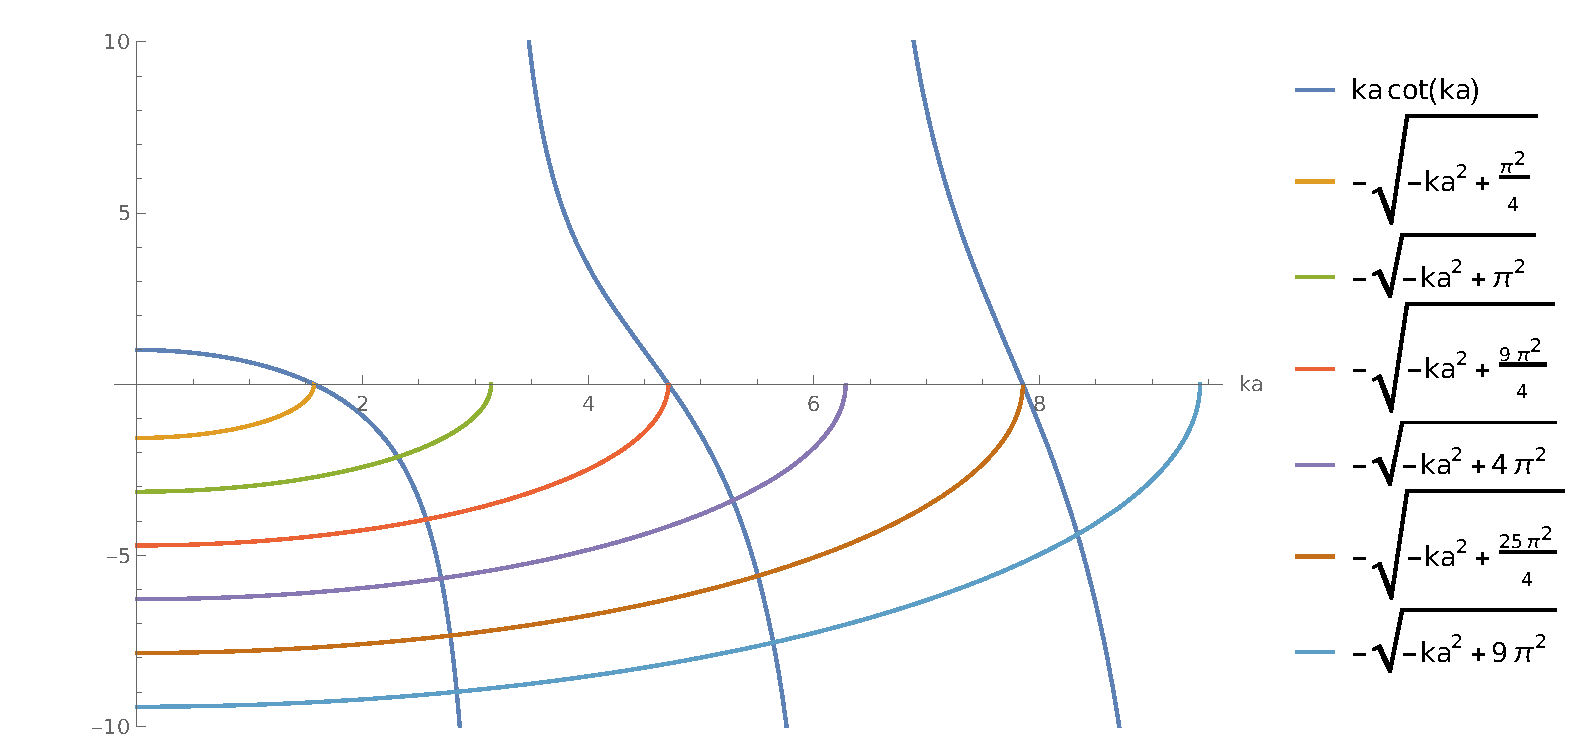
\includegraphics[width=0.75\textwidth]{plot2}
		\caption{Plot demonstrating single bound state solutions to \refeq{ka} in the range $\pi/2 < z < 3\pi/2$, where $z$ is defined in \refeq{kapa}.}
		\label{plot2}
	\end{figure}
	
	Finally, we have the restriction
	\beqn \label{range}
		\frac{\pi}{2} < \sqrt{\frac{2 m \Vo a^2}{\hbar^2}} < \frac{3\pi}{2}
		\qimplies
		\frac{\pi^2 \hbar^2}{8 m a^2} < \Vo < \frac{9\pi^2 \hbar^2}{8 m a^2}.
	\eeqn
	
	The probability for a particle in the bound state to exist outside the well is given by the \hl{transmission coefficient} $T$.
\end{solution}



\begin{problem}
	Consider the scattering problem by the well.  For each $l$, for large enough $r$, when $\Rlr$ is given by
	\beqn \label{outside}
		\Rlr \sim \Al \frac{\sin(kr - l\pi / 2 + \dell)}{r},
	\eeqn
	$\dell$ is called the scattering phase shift.  For the value of $\Vo$ within the range you obtained in the above problem, when the energy of the incident wave is $E = 9 \Vo / 16$, calculate $\tan\delo$~(where $\delo$ is the scattering phase shift for the $s$ wave).
\end{problem}

\begin{solution}
	Now we will use the notation
	\begin{align} \label{kk}
		k' &= \sqrt{\frac{2m (\Vo + E)}{\hbar^2}}, &
		k &= \sqrt{\frac{2m E}{\hbar^2}},
	\end{align}
	where the definition of $k'$ comes from Sakurai (7.7.7),
	\beq
		E + \Vo = \frac{\hbar^2 {k'}^2}{2 m},
	\eeq
	where we have changed the sign of $\Vo$ to fit the notation used here.  These definitions also appear in Sakurai (A.3.2).
	
	We need to match \refeq{outside} with the solution for $r < a$ at the boundary.  In the new notation, the $s$ wave solution for $r < a$ is
	\beqn \label{inside}
		\Ro(r) = \Bo \frac{\sin k' r}{k' r}.
	\eeqn
	Matching \refeq{inside} and \refeq{outside} for $l = 0$ at $r = a$, we obtain
	\beqn \label{cont}
		\Ao \frac{\sin(ka + \delo)}{a} = \Bo \frac{\sin k' a}{k' a}
		\qimplies
		\sin(ka + \delo) = \frac{\Bo}{k' \Ao} \sin k'a.
	\eeqn
	We also need to match the first derivative at the boundary.  Differentiating \refeq{cont}, we find
	\beqn \label{dcont}
		\cos(ka + \delo) = \frac{\Bo}{k \Ao} \cos k'a.
	\eeqn
	Then, dividing \refeq{cont} by \refeq{dcont} gives us
	\beq
		\tan(ka + \delo) = \frac{k}{k'} \tan k'a.
	\eeq
	Using the tangent addition formula
	\beq
		\tan(a + b) = \frac{\tan a + \tan b}{1 - \tan a \tan b},
	\eeq
	we get
	\begin{align}
		\frac{\tan ka + \tan \delo}{1 - \tan ka \tan \delo} &= \frac{k}{k'} \tan k'a \notag \\
		\tan ka + \tan \delo &= \frac{k}{k'} \tan k'a - \frac{k}{k'} \tan k'a \tan ka \tan \delo \notag \\
		\tan \delo \left( 1 + \frac{k}{k'} \tan k'a \tan ka \right) &= \frac{k}{k'} \tan k'a - \tan ka \notag \\
		\tan \delo &= \frac{k \tan k' a - k' \tan ka}{k' + k \tan k' a \tan ka}. \label{delo}
	\end{align}
	
	When the energy of the incident wave is $E = 9 \Vo / 16$,
	\begin{align*}
		k' &= \sqrt{\frac{25 m \Vo}{8 \hbar^2}}, &
		k &= \sqrt{\frac{9 m \Vo}{8 \hbar^2}}, &
		\frac{k}{k'} = \frac{3}{5}.
	\end{align*}
	Using the range of $\Vo$ given by \refeq{range}, we obtain the ranges
	\begin{align*}
		\frac{5 \pi}{8 a} &< k' < \frac{15 \pi}{8 a} &
		\frac{3 \pi}{8 a} &< k < \frac{9 \pi}{8 a}.
	\end{align*}
	Substituting these into \refeq{delo}, the lower bounds give
	\begin{align*}
		\tan\delo &= \frac{3 \tan(5 \pi / 8) - 5 \tan(3\pi / 8)}{5 + 3 \tan(5 \pi / 8) \tan(3\pi / 8)}
		= \frac{-3 (1 + \sqrt{2}) - 5 (1 + \sqrt{2})}{5 - 3 (1 + \sqrt{2}) (1 + \sqrt{2})}
		= \frac{8 (1 + \sqrt{2})}{3(3 + 2 \sqrt{2}) - 5}
		= \frac{4 + 4 \sqrt{2}}{2 + 3 \sqrt{2}} \frac{2 - 3 \sqrt{2}}{2 - 3 \sqrt{2}} \\
		&= \frac{4 \sqrt{2} + 16}{14}
		= \frac{\sqrt{8} + 8}{7},
	\end{align*}
	and the upper bounds give
	\begin{align*}
		\tan\delo &= \frac{3 \tan(15 \pi / 8) - 5 \tan(9\pi / 8)}{5 + 3 \tan(15 \pi / 8) \tan(9\pi / 8)}
		= \frac{3 (1 - \sqrt{2}) + 5 (1 - \sqrt{2})}{5 - 3 (1 - \sqrt{2}) (1 - \sqrt{2})}
		= \frac{8 (1 - \sqrt{2})}{5 - 3 (3 - 2 \sqrt{2})}
		= \frac{4 - 4 \sqrt{2}}{3 \sqrt{2} - 2} \frac{2 + 3 \sqrt{2}}{2 + 3 \sqrt{2}} \\
		&= \frac{4 \sqrt{2} - 16}{14}
		= \frac{\sqrt{8} - 8}{7}.
	\end{align*}
	So we have the range
	\beq
		\frac{\sqrt{8} - 8}{7} < \tan\delo < \frac{\sqrt{8} + 8}{7}.
	\eeq
	\vfix
\end{solution}



\begin{problem}
	Now consider the $S$ matrix, $S \equiv e^{2i \delo} = e^{i \delo} / e^{-i \delo}$.  Compare the condition on $s$ wave bound state energies and the zero of the denominator of $S$.  Explain their relation.
\end{problem}

\begin{solution}
	$S$ has a pole on the imaginary axis when
	\beq
		0 = \Re[e^{-i \delo}] = \Re[\cos\delo - i \sin\delo] = \cos\delo
		\qimplies
		\delo = n\pi + \frac{\pi}{2}, \quad n = 0, 1, 2, \ldots.
	\eeq
	This is similar to the condition we saw for bound state energies in \ref{2.2}.  As displayed in Fig.~\ref{plot2}, the $(n + 1)$th bound state appears when $z = n\pi + \pi / 2$.  From the definition of $z$ in \refeq{kapa}, there are $(n + 1)$ possible bound states when
	\beq
		\sqrt{\frac{2 m \Vo a^2}{\hbar^2}} > n\pi + \frac{\pi}{2}, \quad n = 0, 1, 2, \ldots,
	\eeq
	which gives a relationship between $\Vo$, the depth of the potential well, and the $\delo$ corresponding to the poles of $S$.  As we increase the depth of the potential well, we move along the imaginary axis, and an additional bound state is possible for every pole we cross.
\end{solution}

%	From (7.6.35) in Sakurai,
%	\beqn \label{dell}
%		\tan\dell = \frac{k a \jl'(ka) - \betal \jl(ka)}{k a \nl'(ka) - \betal \nl(ka)},
%	\eeqn
%	where (7.6.34) defines $\betal$,
%	\beq
%		\betal \equiv \left[ \frac{r}{\Rl} \dv{\Rl}{r} \right]_{r=a},
%	\eeq
%	$\nl$ are the Neumann functions, given by (A.5.12),
%	\beq
%		\nl(\rho) = (-1)^{l+1} \sqrt{\frac{\pi}{2\rho}} J_{-l-1/2}(\rho),
%	\eeq
%	and
%	\begin{align*}
%		\jl'(ka) &= \left. \dv{\jl}{(kr)} \right|_{kr = ka}, &
%		\nl'(ka) &= \left. \dv{\nl}{(kr)} \right|_{kr = ka}.
%	\end{align*}
%	
%	For $\betao$, applying \refeq{Rl} and \refeq{jo} gives us
%	\begin{align*}
%		\frac{r}{\Ro} \dv{\Ro}{r} &= \frac{r}{\jo(kr)} \dv{\jo(kr)}{r}
%		= \frac{kr^2}{\sin kr} \dv{r} \!\left( \frac{\sin kr}{kr} \right)
%		= \frac{kr^2}{\sin kr} \left[ \frac{1}{kr} \dv{r} (\sin kr) + \sin kr \dv{r}\! \left( \frac{1}{kr} \right) \right] \\
%		&= \frac{kr^2}{\sin kr} \left( \frac{\cos kr}{r} - \frac{\sin kr}{k r^2} \right)
%		= kr \cot kr - 1.
%	\end{align*}
%	Once again applying \refeq{jo}, note that
%	\beq
%		\dv{\jo}{(kr)} = \dv{(kr)} \!\left( \frac{\sin kr}{kr} \right)
%		= \frac{1}{kr} \dv{(kr)} (\sin kr) + \sin kr \dv{(kr)} \!\left( \frac{1}{kr} \right)
%		= \frac{\cos kr}{kr} - \frac{\sin kr}{k^2 r^2}
%		= \frac{kr \cos kr - \sin kr}{k^2 r^2}.
%	\eeq
%	From Sakurai (A.5.12),
%	\beq
%		\no(\rho) = -\frac{\cos\rho}{\rho}
%	\eeq
%	so
%	\beq
%		\dv{\no}{(kr)} = \dv{(kr)} \!\left( -\frac{\cos kr}{kr} \right)
%		= -\frac{1}{kr} \dv{(kr)} (\cos kr) - \cos kr \dv{(kr)} \!\left( \frac{1}{kr} \right)
%		= \frac{\sin kr}{kr} + \frac{\cos kr}{k^2 r^2}
%		= \frac{kr \sin kr + \cos kr}{k^2 r^2}.
%	\eeq
%	
%	Making these substitutions into \refeq{dell},
%	\begin{align*}
%		\tan \delo &= \left[ ka \frac{ka \cos ka - \sin ka}{k^2 a^2} - (ka \cot ka - 1) \frac{\sin ka}{ka} \right] \left[ ka \frac{ka \sin ka + \cos ka}{k^2 a^2} + (ka \cot ka - 1) \frac{\cos ka}{ka} \right]^{-1} \\
%		&= \frac{ka \cos ka - \sin ka - (ka \cot ka - 1) \sin ka}{ka \sin ka + \cos ka + (ka \cot ka - 1) \cos ka}
%		= 0.
%	\end{align*}